\documentclass[border=20pt]{standalone}
\usepackage{tikz}
\usetikzlibrary{arrows.meta, positioning, calc}

\begin{document}
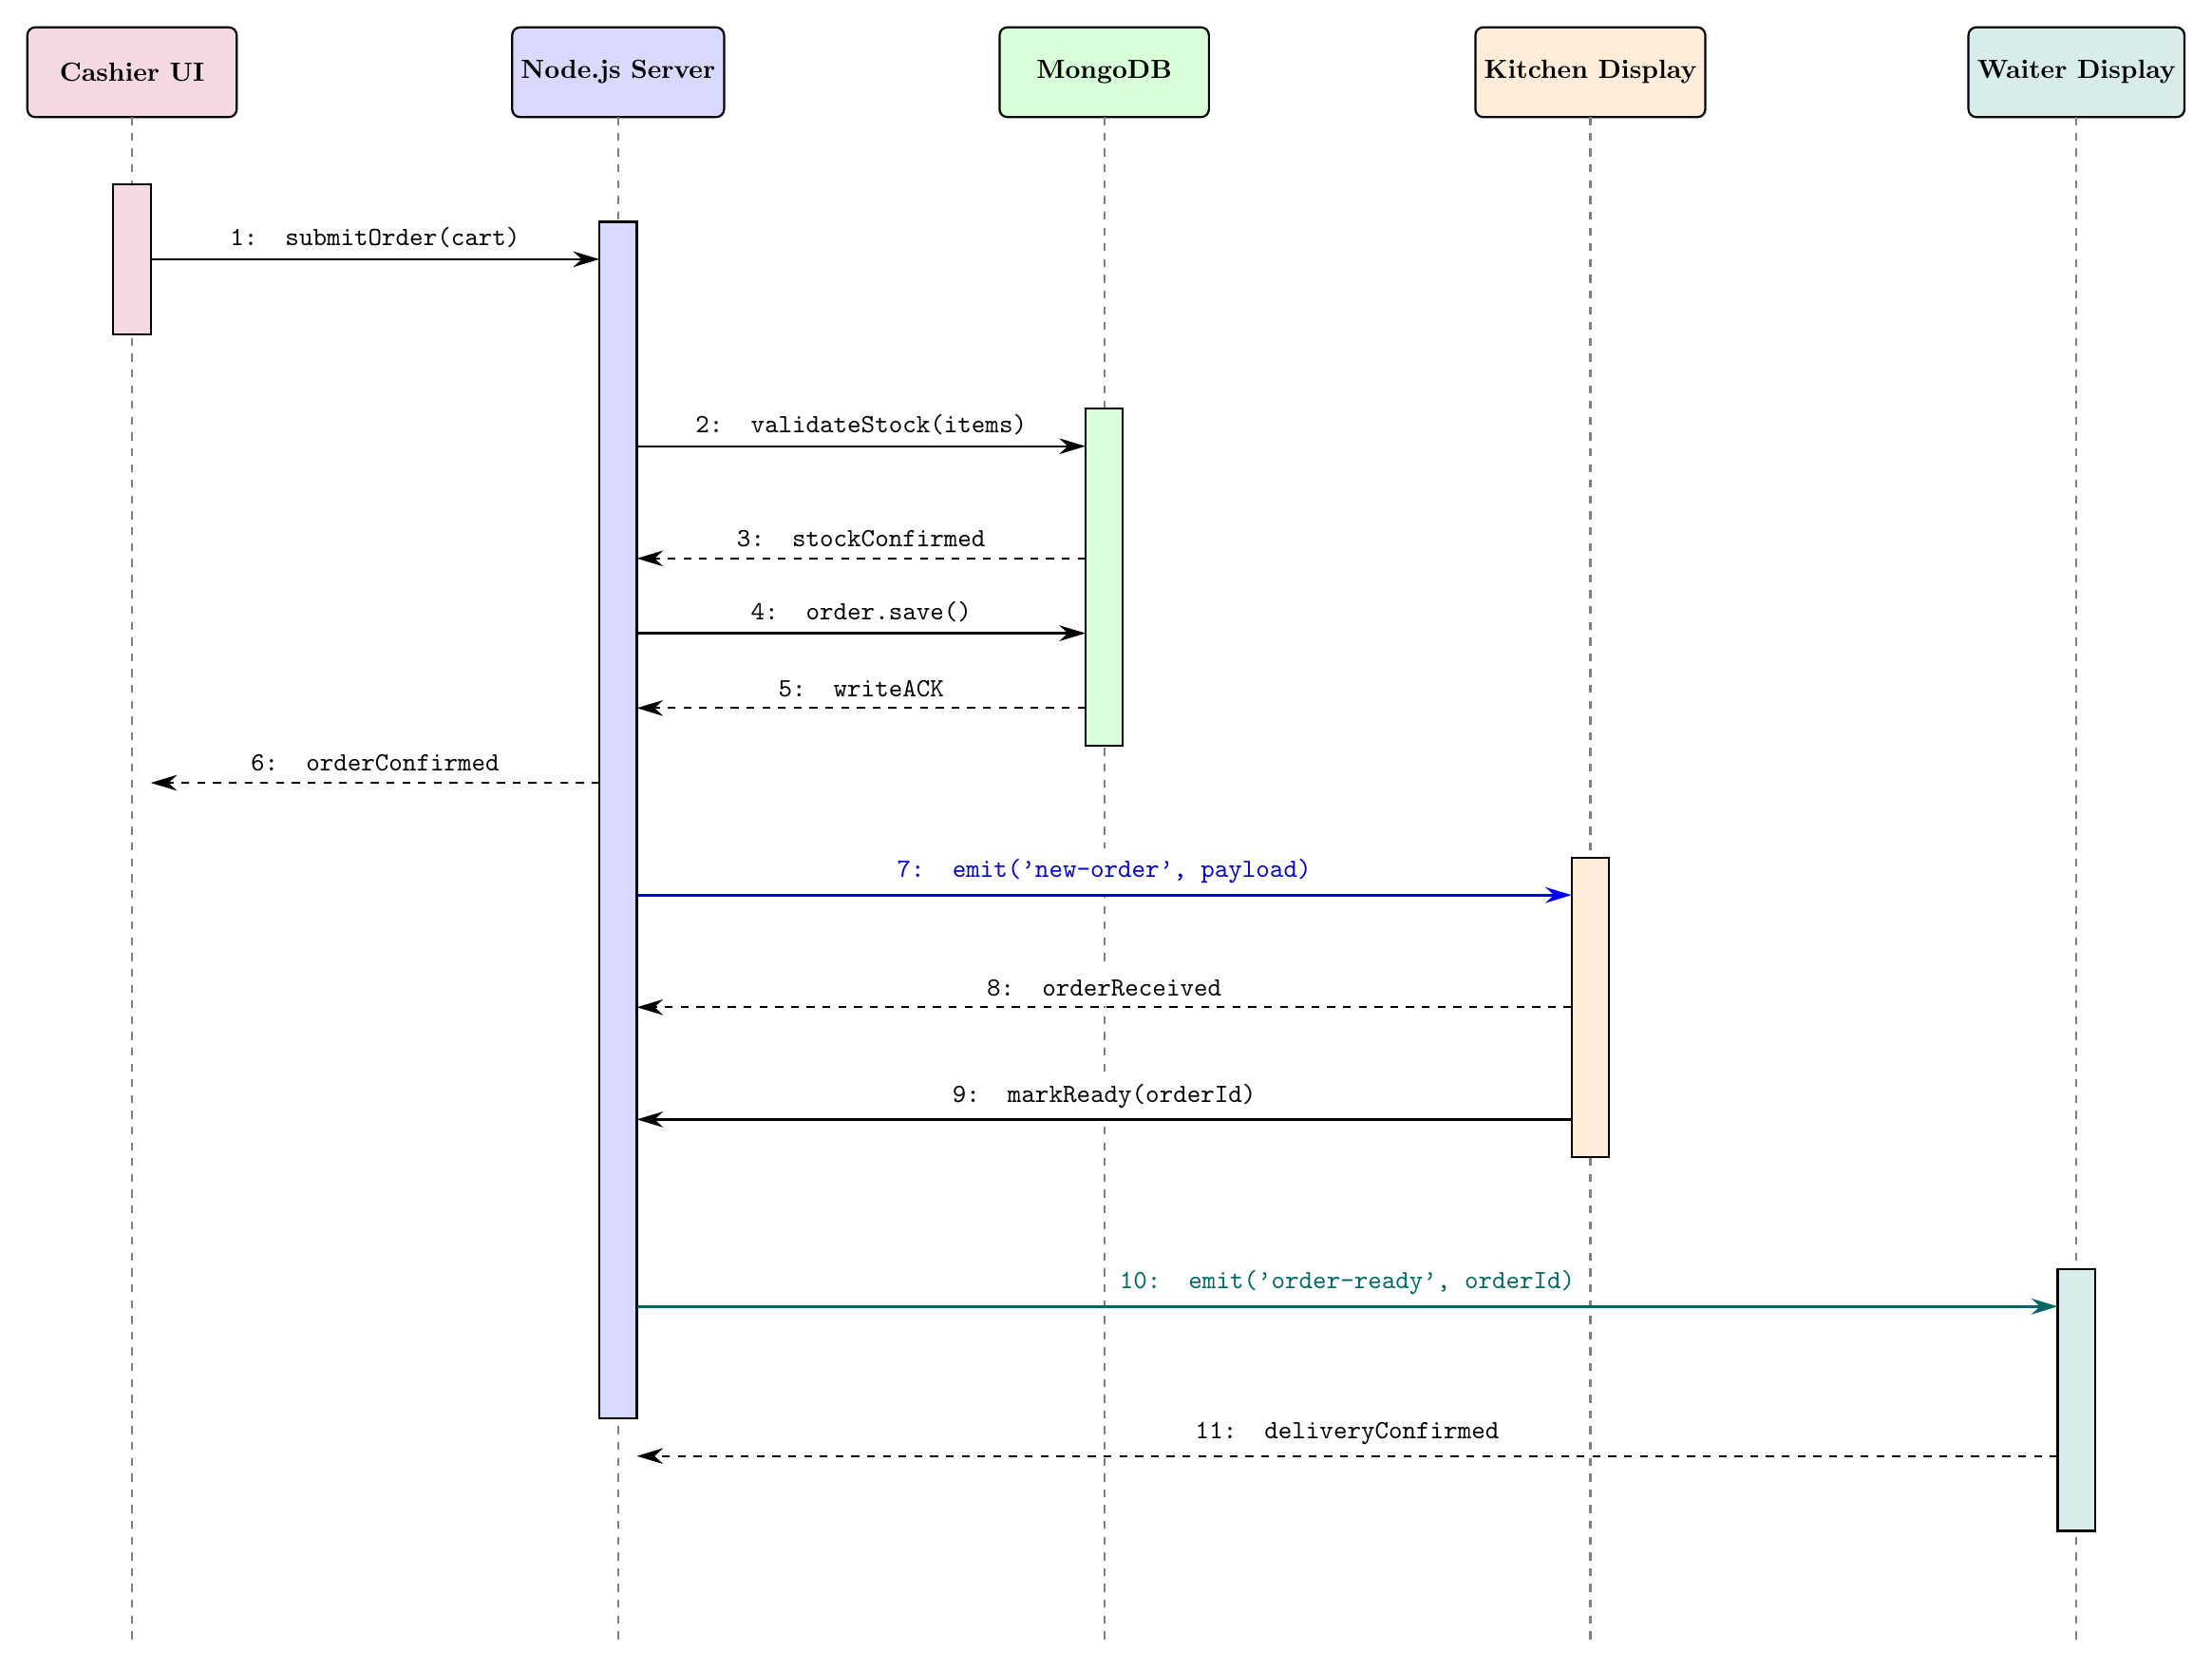
\begin{tikzpicture}[
    entity/.style={draw, rectangle, minimum width=2.8cm, minimum height=1.2cm, align=center, font=\normalsize\bfseries, fill=#1, rounded corners=3pt, thick},
    entity/.default=blue!10,
    msg/.style={-{Stealth[length=10pt, width=6pt]}, thick},
    dashmsg/.style={-{Stealth[length=10pt, width=6pt]}, dashed, thick},
    msglabel/.style={font=\normalsize\ttfamily, fill=white, inner sep=4pt, midway, above},
    lifeline/.style={dashed, gray, thick},
    activation/.style={draw, fill=#1, minimum width=0.5cm, thick},
    activation/.default=blue!10
]

% --- Entities ---
\node[entity=purple!15] (cashier) at (0, 0) {Cashier UI};
\node[entity=blue!15]   (server)  at (6.5, 0) {Node.js Server};
\node[entity=green!15]  (mongo)   at (13, 0) {MongoDB};
\node[entity=orange!15] (kitchen) at (19.5, 0) {Kitchen Display};
\node[entity=teal!15]   (waiter)  at (26, 0) {Waiter Display};

% --- Lifelines ---
\foreach \x in {0, 6.5, 13, 19.5, 26} {
    \draw[lifeline] (\x, -0.6) -- (\x, -21);
}

% --- Activation bars ---
% Cashier: 0 to 0.5 (Centered around 0 is actually -0.25 to 0.25, let's just draw them shifted right)
\draw[activation=purple!15] (-0.25, -1.5) rectangle (0.25, -3.5);
\draw[activation=blue!15]   (6.25, -2.0) rectangle (6.75, -18.0);
\draw[activation=green!15]  (12.75, -4.5) rectangle (13.25, -9.0);
\draw[activation=orange!15] (19.25, -10.5) rectangle (19.75, -14.5);
\draw[activation=teal!15]   (25.75, -16.0) rectangle (26.25, -19.5);

% X coordinates for arrows
\def\Cr{0.25} % Cashier right
\def\Sl{6.25} % Server left
\def\Sr{6.75} % Server right
\def\Ml{12.75} % Mongo left
\def\Mr{13.25} % Mongo right
\def\Kl{19.25} % Kitchen left
\def\Kr{19.75} % Kitchen right
\def\Wl{25.75} % Waiter left

% --- Messages ---

% 1. Cashier submits order
\draw[msg] (\Cr, -2.5) -- node[msglabel] {1: submitOrder(cart)} (\Sl, -2.5);

% 2. Server validates stock
\draw[msg] (\Sr, -5.0) -- node[msglabel] {2: validateStock(items)} (\Ml, -5.0);

% 3. MongoDB confirms
\draw[dashmsg] (\Ml, -6.5) -- node[msglabel] {3: stockConfirmed} (\Sr, -6.5);

% 4. Server persists order
\draw[msg] (\Sr, -7.5) -- node[msglabel] {4: order.save()} (\Ml, -7.5);

% 5. MongoDB ACK
\draw[dashmsg] (\Ml, -8.5) -- node[msglabel] {5: writeACK} (\Sr, -8.5);

% 6. Server confirms to cashier
\draw[dashmsg] (\Sl, -9.5) -- node[msglabel] {6: orderConfirmed} (\Cr, -9.5);

% 7. Server emits to kitchen
\draw[msg, draw=blue, very thick] (\Sr, -11.0) -- node[msglabel, text=blue!80!black] {7: emit('new-order', payload)} (\Kl, -11.0);

% 8. Kitchen acknowledges
\draw[dashmsg] (\Kl, -12.5) -- node[msglabel] {8: orderReceived} (\Sr, -12.5);

% 9. Cook marks order ready
\draw[msg] (\Kl, -14.0) -- node[msglabel] {9: markReady(orderId)} (\Sr, -14.0);

% 10. Server notifies waiter
\draw[msg, draw=teal!80!black, very thick] (\Sr, -16.5) -- node[msglabel, text=teal!80!black] {10: emit('order-ready', orderId)} (\Wl, -16.5);

% 11. Waiter confirms delivery
\draw[dashmsg] (\Wl, -18.5) -- node[msglabel] {11: deliveryConfirmed} (\Sr, -18.5);

\end{tikzpicture}
\end{document}
